% Created 2022-05-12 Thu 16:17
% Intended LaTeX compiler: pdflatex
\documentclass[11pt]{article}
\usepackage[utf8]{inputenc}
\usepackage[T1]{fontenc}
\usepackage{graphicx}
\usepackage{longtable}
\usepackage{wrapfig}
\usepackage{rotating}
\usepackage[normalem]{ulem}
\usepackage{amsmath}
\usepackage{amssymb}
\usepackage{capt-of}
\usepackage{hyperref}
\author{Ali, Mihir, Noah}
\date{\today}
\title{Einführung in die Theoretische Informatik Zusammenfassung}
\hypersetup{
 pdfauthor={Ali, Mihir, Noah},
 pdftitle={Einführung in die Theoretische Informatik Zusammenfassung},
 pdfkeywords={},
 pdfsubject={},
 pdfcreator={Emacs 28.1 (Org mode 9.6)}, 
 pdflang={English}}
\begin{document}

\maketitle
\tableofcontents


\section{Formale Sprachen}
\label{sec:orgf1aba2b}

\subsection{Grundbegriffe}
\label{sec:org865717d}
\begin{itemize}
\item Alphabet \(\Sigma\) (endliche Menge) z.B. \(\{1,0\}\)
\item Wort/String über \(\Sigma\) ist eine endliche Folge von Zeichen aus \(\Sigma\)
\item \(|w|\) länge des Wortes \(w\)
\item Leeres Wort \(\epsilon\)
\item \(uv\) konkatenation der Wörter \(u\) und \(w\)
\item Ist \(w\) ein Wort so ist \(w^0 = \epsilon\) und \(w^{n+1} = ww^n\)
\item \(\Sigma^*\) Menge aller Wörter über \(\Sigma\)
\item (formale) Sprache \(L \subseteq \Sigma^*\)
\end{itemize}

\subsubsection{Operationen auf Sprachen}
\label{sec:orgee69c64}
Seien \(A,B \subseteq \Sigma^*\)
\begin{itemize}
\item Konkatenation:
\end{itemize}
\(AB = \{uv | u \in A \land v \in B \}\)
\begin{itemize}
\item Konkatenation mit sich selbst:
\end{itemize}
\(A^n = \{w_1 ... w_n | w_1, ... , w_n \in A\} = A ... A\)
\begin{itemize}
\item \(A^* = \{w_1...w_n | n \geq 0 \land w_1, ... , w_n \in A\} = \bigcup_{n\in \mathbb{N}} A^n\)
\item \(A^+ = AA^* = \bigcup_{n \geq 1} A^n\)
\end{itemize}
\begin{enumerate}
\item Sonderfälle:
\label{sec:org9c3334e}
\begin{itemize}
\item \(\forall A: \epsilon \in A^*\)
\item \(\emptyset^* = \{\epsilon\}\)
\item \(\emptyset A = \emptyset\)
\item \(\{\epsilon \} A = A\)
\item \(A^*A^* = A^* = (A^*)^*\)
\end{itemize}
\end{enumerate}

\subsubsection{Grammatiken}
\label{sec:org725c5c6}
4-Tupel \(G = (V,\Sigma,P,S)\)
\begin{itemize}
\item \(V\) ist endliche Menge von Nichtterminalzeichen
\item \(\Sigma\) ist endliche Menga von Terminalzeichen (= Alphabet)
\item \(P \subseteq (V \cup \Sigma)^* \times (V \cup \Sigma)^*\) ist Menge von Produktionen
\item \(S \in V\) ist das Startsymbol
\end{itemize}

Die Sprache von G ist die Menge aller Wörter, die von G erzeugt werden. Sie wird mit \(L(G)\) bezeichnet.
Also jedes Wort, dass die Grammatik erzeugt muss in der Sprache erhalten sein und jedes Wort in der Sprache muss von der Grammatik erzeugt werden.
\begin{enumerate}
\item Reflexve transitive Hülle
\label{sec:org4274eb2}

\begin{itemize}
\item \(\alpha \rightarrow^0_G \alpha\)
\item \(\alpha \rightarrow^{n+1}_G \gamma: \exists \beta. \alpha \rightarrow^n_G \rightarrow_G \gamma\)
\item \(\alpha \rightarrow^{*}_G \beta : \exists n. \alpha \rightarrow^n_G \beta\)
\item \(\alpha \rightarrow^{+}_G \beta: \exists n>0. \alpha \rightarrow^n_G \beta\)
\end{itemize}
\end{enumerate}

\subsubsection{Chomsky Hierarchie}
\label{sec:orgb9c5b31}
Eine Grammatik G ist vom
\begin{itemize}
\item Typ 0 immer
\item Typ 1 falls fpr jede Produktion \(\alpha \rightarrow \beta\) außer \(S \rightarrow \epsilon\) gilt \(|\alpha| \leq |\beta|\)
\item Typ 2 Falls G vom typ 1 ist und für jede Produktion \(\alpha \righarrow \beta\) gilt \(\alpha \in V\)
\item Typ 3 falls G vom Typ 2 ist und für jede Produktion \(\alpha \rightarrow \beta\) außer \(S \rightarrow \epsilon\) gilt \(\beta \in \Sigma \cup \Sigma V\)
\end{itemize}

\begin{enumerate}
\item Grmmatiken und Sprachklassen:
\label{sec:org8b931ed}
\begin{center}
\begin{tabular}{lll}
Typ 3 & Rechtslineare Grammatiken & Reguläre Sprachen\\
Typ 2 & Kontextfreie Grammatik & Kontextfreie Sprachen\\
Typ 1 & Kontextsensitive Grammatik & Kontextsens. Sprachen\\
Typ 0 & Phrasenstrukturgrammatik & Rekursiv aufzählbare Sprachen\\
\end{tabular}
\end{center}

\item Satz 2.13
\label{sec:orgf67a500}
\(L(Typ 3) \subset L(Typ 2) \subset L(Typ 1) \subset L(Typ 0)\)
\end{enumerate}

\subsubsection{Wortproblem}
\label{sec:org26c819d}
Gegeben: eine Grammatik G, ein Wort \(w \in \Sigma^*\)
Frage: Ist das Wort in w enthalten (\(w \in L(G)\))?

\section{Reguläre Sprachen}
\label{sec:orgc6a1e7c}

\begin{figure}[htbp]
\centering
\includegraphics[width=.9\linewidth]{./img/2-kapitel/reguläre_sprachen.png}
\caption{Reguläre Sprachen Schema}
\end{figure}

\subsection{Deterministische endliche Automaten}
\label{sec:orgae1f75f}
\begin{figure}[htbp]
\centering
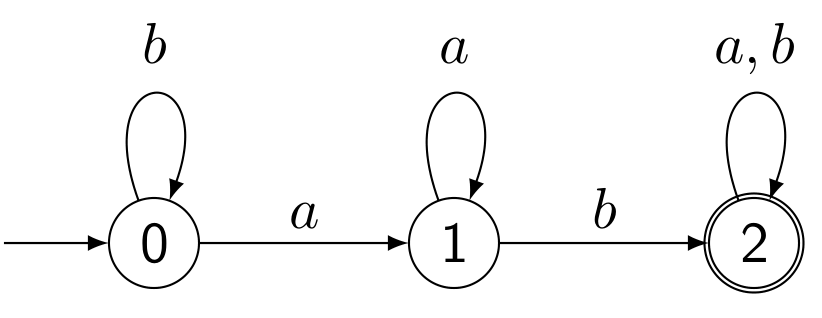
\includegraphics[width=.9\linewidth]{./img/2-kapitel/automat_bsp.png}
\caption{Beispiel Automat}
\end{figure}

\begin{itemize}
\item Beispiel:
\begin{itemize}
\item Eingabewort \(baba \rightarrow\) Zustandsfolge 0,0,1,2,2
\end{itemize}
\item ``Bei dieser Grammatik muss mindestens nach einem a ein b kommen''
\item Die Sprache des DFA ist die Menge aller Wörter über \(\{a,b\}\), die ab enthalten
\end{itemize}

Erkannte Sprache: Menge der Wörter, die vom Startzustand in einen Endzustand führen.
Recognizer, die nur einmal das Wort durchläuft und in linearer Zeit es akzeptiert oder ablehnt.

\subsubsection{Definition}
\label{sec:org859d242}
Ein deterministischer endlicher Automat \(M = (Q,\Sigma, \delta, q_0, F)\) besteht aus
\begin{itemize}
\item endliche Menge von Zuständen Q
\item endlichem Eingabealphabet \(\Sigma\)
\item einer totalen Übergangsfunktion \(\delta: Q \times \Sigma \rightarrow Q\)
\item eienm Startzustand \(q_0 \in Q\)
\item einer Menge \(F \subset Q\) von Endzuständen
\end{itemize}

\begin{enumerate}
\item Akzeptierte Sprachen (Definition 3.2)
\label{sec:org0b94072}
Von M akzeptierte Sprache \(L(M) := \{w \in \Sigma^* | \hat{\delta}(q_0, w) \in F\}\) wobei \\
\(\hat{\delta}: Q \times \Sigma^* \rightarrow Q\) induktiv definiert ist: \\
\(\hat{\delta}(q,\epsilon) = q\) \\
\(\hat{\delta}(q,aw) = \hat{\delta}(\delta(q,a),w)\), für \(a \in \Sigma, w \in \Sigma^*\) \\
(\(\hat{\delta}(q, w)\) bezeichnet den Zustand, den man aus \(q\) mit \(w\) erreicht.)\\
Eine Sprache ist regulär \textbf{gdw} sie von einem DFA akzeptiert wird.

\item Beispiel Automat der Sprache akzeptiert
\label{sec:orgd43d4d4}
Induktiv beweisen pro Zustand.
\end{enumerate}


\subsection{Von rechtslinearen Grammatiken zu DFA}
\label{sec:orgf976173}
\begin{itemize}
\item Für jede rechtslineare Grammatik \(G\) gibt es einen DFA \(M\) mit \(L(M) = L(G)\)
\item Für jeden DFA \(M\) gibt es eine rechtslineare Grammatik \(G\) mit \(L(G) = L(M)\)
\end{itemize}

\subsubsection{Nichtdeterministischer endlicher Automat}
\label{sec:orgee625c9}
Ein deterministischer endlicher Automat \(M = (Q,\Sigma, \delta, q_0, F)\) besteht aus
\begin{itemize}
\item \(Q, \Sigma, q_0, F\) sind wie DFA
\item \(\delta: Q \times \Sigma \rightarrow P(Q)\) \\
\(P(Q)\) = Menge aller Teilmengen von \(Q = 2^Q\) \\
Alternative: Relation \(\delta \subseteq Q \times \Sigma \times Q\)
\end{itemize}


\(\bar{\delta}(S,a) := \bigcup_{q \in S} \delta(q,a)\)


Es folgt: \(\hat{\bar{\delta}}: P(Q) \times \Sigma^* \rightarrow P(Q)\)

\begin{enumerate}
\item Intuition:
\label{sec:org55b81d1}
\(\hat{\bar{\delta}}(S,w)\) ist Menge aller Zustände, die sich von einem Zustand in S aus \(w\) erreichen lassen.

\item Von nichtdeterminitsichen Automaten N akzeptierte Sprache
\label{sec:org27506eb}
\(L(N) := \{w \in \Sigma^* | \hat{\bar{\delta}}(\{q_0\},w) \cap F \neq \emptyset\}\)
\end{enumerate}

\subsubsection{Satz 3.9}
\label{sec:org77d34b9}
Für jede rechtslineare Grammatik G gibt es einen NFA M mit \(L(G) = L(M)\)
\subsubsection{Satz 3.13}
\label{sec:org81405bb}
Für jeden DFA M gibt es eine rechtslineare Grammatik G mit \(L(M) = L(G)\)

\subsection{3.3 NFAs mit \(\epsilon\) -Übergängen}
\label{sec:orgd2dc9c9}
Grammatiken von Programmiersprachen enthalten viele Produktionen der Gestalt \(A \rightarrow B\).

Ein NFA mit \textbf{\(\epsilon\)}-Übergängen (auch \(\epsilon\) -NFA) ist ein NFA mit einem speziellen Symbol \(\epsilon \not \in \Sigma\) und mit
\(\delta : Q \times (\Sigma \cup {\epsilon}) \rightarrow P(Q)\) .
Ein \(\epsilon\) übergang darf ausgef¨uhrt werden, ohne dass ein

\subsubsection{Lemma 3.16}
\label{sec:org0f23773}
Für jeden \(\epsilon\) -NFA \(N\) gibt es einen NFA \(N'\) mit \(L(N) = L(N')\).

\subsection{3.4 Regex}
\label{sec:org9f1a132}
\begin{itemize}
\item \(\emptyset\) ist ein regex
\item \(\epsilon\) ist ein regex
\item Für jedes \(a \in \Sigma\) ist a ein regulärer Audruck
\item Wenn \(\alpha\) und \(\beta\) regex dann auch
\begin{enumerate}
\item \(\alpha \beta\)
\item \(\alpha | \beta\)
\item \(\alpha^*\)
\end{enumerate}
\item Sonst NIX!
\end{itemize}
\subsubsection{Definition 3.20}
\label{sec:org6a58dac}
Zu einem regulären Ausdruck \(\gamma\) ist die zugehörige Sprache \(L(\gamma)\) rekursiv definiert:
\begin{itemize}
\item \(L(\emptyset) =\emptyset\)
\item \(L(\epsilon) = \{\epsilon\}\)
\item \(L(a) = {a}\)
\item \(L(\alpha \beta) = L(\alpha)L(\beta))\)
\item \(L(\alpha | \beta) = L(\alpha) \cup L(\beta)\)
\item \(L(\alpha^*) = L(\alpha)^*\)
\end{itemize}
\subsubsection{Satz 3.23 (Kleene 1956)}
\label{sec:orge873ff1}
Eine Sprache \(L \subseteq \Sigma^*\) ist genau dann durch einen regulären Ausdruck darstellbar, wenn sie regulär ist.

\subsubsection{Wie teuer sind unsere Konversionen?}
\label{sec:orgee842a8}
\begin{center}
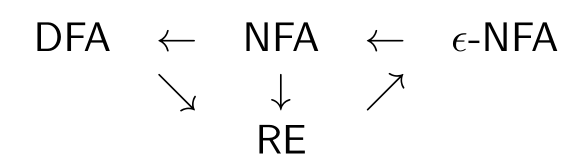
\includegraphics[width=.9\linewidth]{./img/2-kapitel/konversionen.png}
\end{center}
\begin{itemize}
\item RE \(\rightarrow \epsilon\) -NFA: RE der Länge n, \(O(n)\) Zustände
\item \(\epsilon\) -NFA \(\rightarrow\) NFA: Q
\item NFA \(\rightarrow\) DFA: \(O(2^n)\)
\item FA \(\rightarrow\) RE: \(O(n4^n)\)
\end{itemize}

\subsection{Abschlusseigenschaften regulärer Sprachen}
\label{sec:org808654e}
\subsubsection{Satz 3.24}
\label{sec:org25400fa}
Seien \(R,R_1, R_2 \subseteq \Sigma^*\) reguläre Sprachen. Dann sind auch
\begin{itemize}
\item \(R_1R_2\)
\item \(R_1 \cup R_2\)
\item \(R^*\)
\item \(\bar{R} (:= \Sigma^* \backslash R)\)
\item \(R_1 \cup R_2\)
\item \(R_1 \backslash R_2\) \\
\end{itemize}
reguläre Sprachen

\begin{enumerate}
\item Produkt-Konstruktion
\label{sec:orgac3fd2a}
Für den Schnitt ist die De-Morgan regel zu teuer also kann man auch eine Produkt Konstruktion ohne Umweg über De-Morgen benutzen.

Das funktioniert über Parallelismus also beide DFAs laufen synchron parallel (kreuzprodukt der Zustandsräume).
\end{enumerate}

\subsection{Rechnen mit Regulären Ausdrücken}
\label{sec:org8ca1c8d}
\subsubsection{Definition 3.26}
\label{sec:orge2fcf73}
Zwei reguläre Ausdrücke sind \textbf{äquivalent gdw} sie die gleiche Sprache darstellen:
\(\alpha \equiv \beta: \Leftrightarrow L(\alpha) = L(\beta)\)

(by the way \(\equiv\) steht für Bedeutungsäquivalenz und \(=\) für syntaktische gleichheit)

\subsection{Pumping Lemma}
\label{sec:org4fb520b}
Wie zeigt man, dass eine Sprache nicht regulär ist?
\subsubsection{Satz 3.32 (Pumping Lemma für Reguläre Sprachen)}
\label{sec:orgae43e3f}
Sei \(R \subseteq \Sigma^*\) regulär. Dann gibt es ein \(n > 0\), so dass sich jedes \(z \in R\) mit \(|z| \geq n\) so in \(z = uvw\) zerlegen lässt, dass
\begin{itemize}
\item \(v \neq \epsilon\),
\item \(|uv| \leq n\)
\item \(\forall i \geq 0. uv^iw \in R\). \\
\end{itemize}

Es gibt nicht-reguläre Sprachen, für die das Pumping-Lemma gilt!
\(\Rightarrow\) Pumping-Lemma hinreichend aber nicht notwendig um Nicht-Regularität zu zeigen.

regulär  \(\subset\) Pumping-Lemma gilt \(\subset\) alle Sprachen

\subsection{Entscheidungsverfahren}
\label{sec:orgead09db}

\textbf{Eingabe:} Ein oder mehrere Objekte, die Reguläre Sprachen beschreiben (DFA, NFA, RE Typ3 Gram, \ldots{})
\textbf{Frage:} Haben die Sprachen die Eigenschaft X?
Ein (Entscheidungs-)Problem ist entscheidbar, wenn es einen Algorithmus gibt, der bei jeder Eingabe in endlicher Zeit die richtige Antwort auf die Frage feststellt.

Welche Entscheidungsprobleme sind für rechtslineare Grammatiken entscheidbar und wie hängt die Laufzeit mit der Beschreibung zusammen.

\subsubsection{Definition 3.37}
\label{sec:orgaa917eb}
Sei D ein DFA, NFA, RE, rechtslineare Grammatik \ldots{}
\begin{itemize}
\item \textbf{Wortproblem}: Gegeben \(w\) und D: gilt \(w \in L(D)\)
\item \textbf{Leerheitsproblem}: Gegeben D: gilt \(\emptyset = L(D)\)
\item \textbf{Endlichkeitsproblem}: Gegeben D: isz \(L(D)\) endlich
\item \textbf{Äquivalenzproblem}: Gegeben \(D_1, D_2\), gilt \(L(D_1) = L(D_2)\)
\end{itemize}
\end{document}
